\begin{frame}
\frametitle{Table et actions à réaliser}
\framesubtitle{Table}
\begin{figure}[!ht]
	\centering
	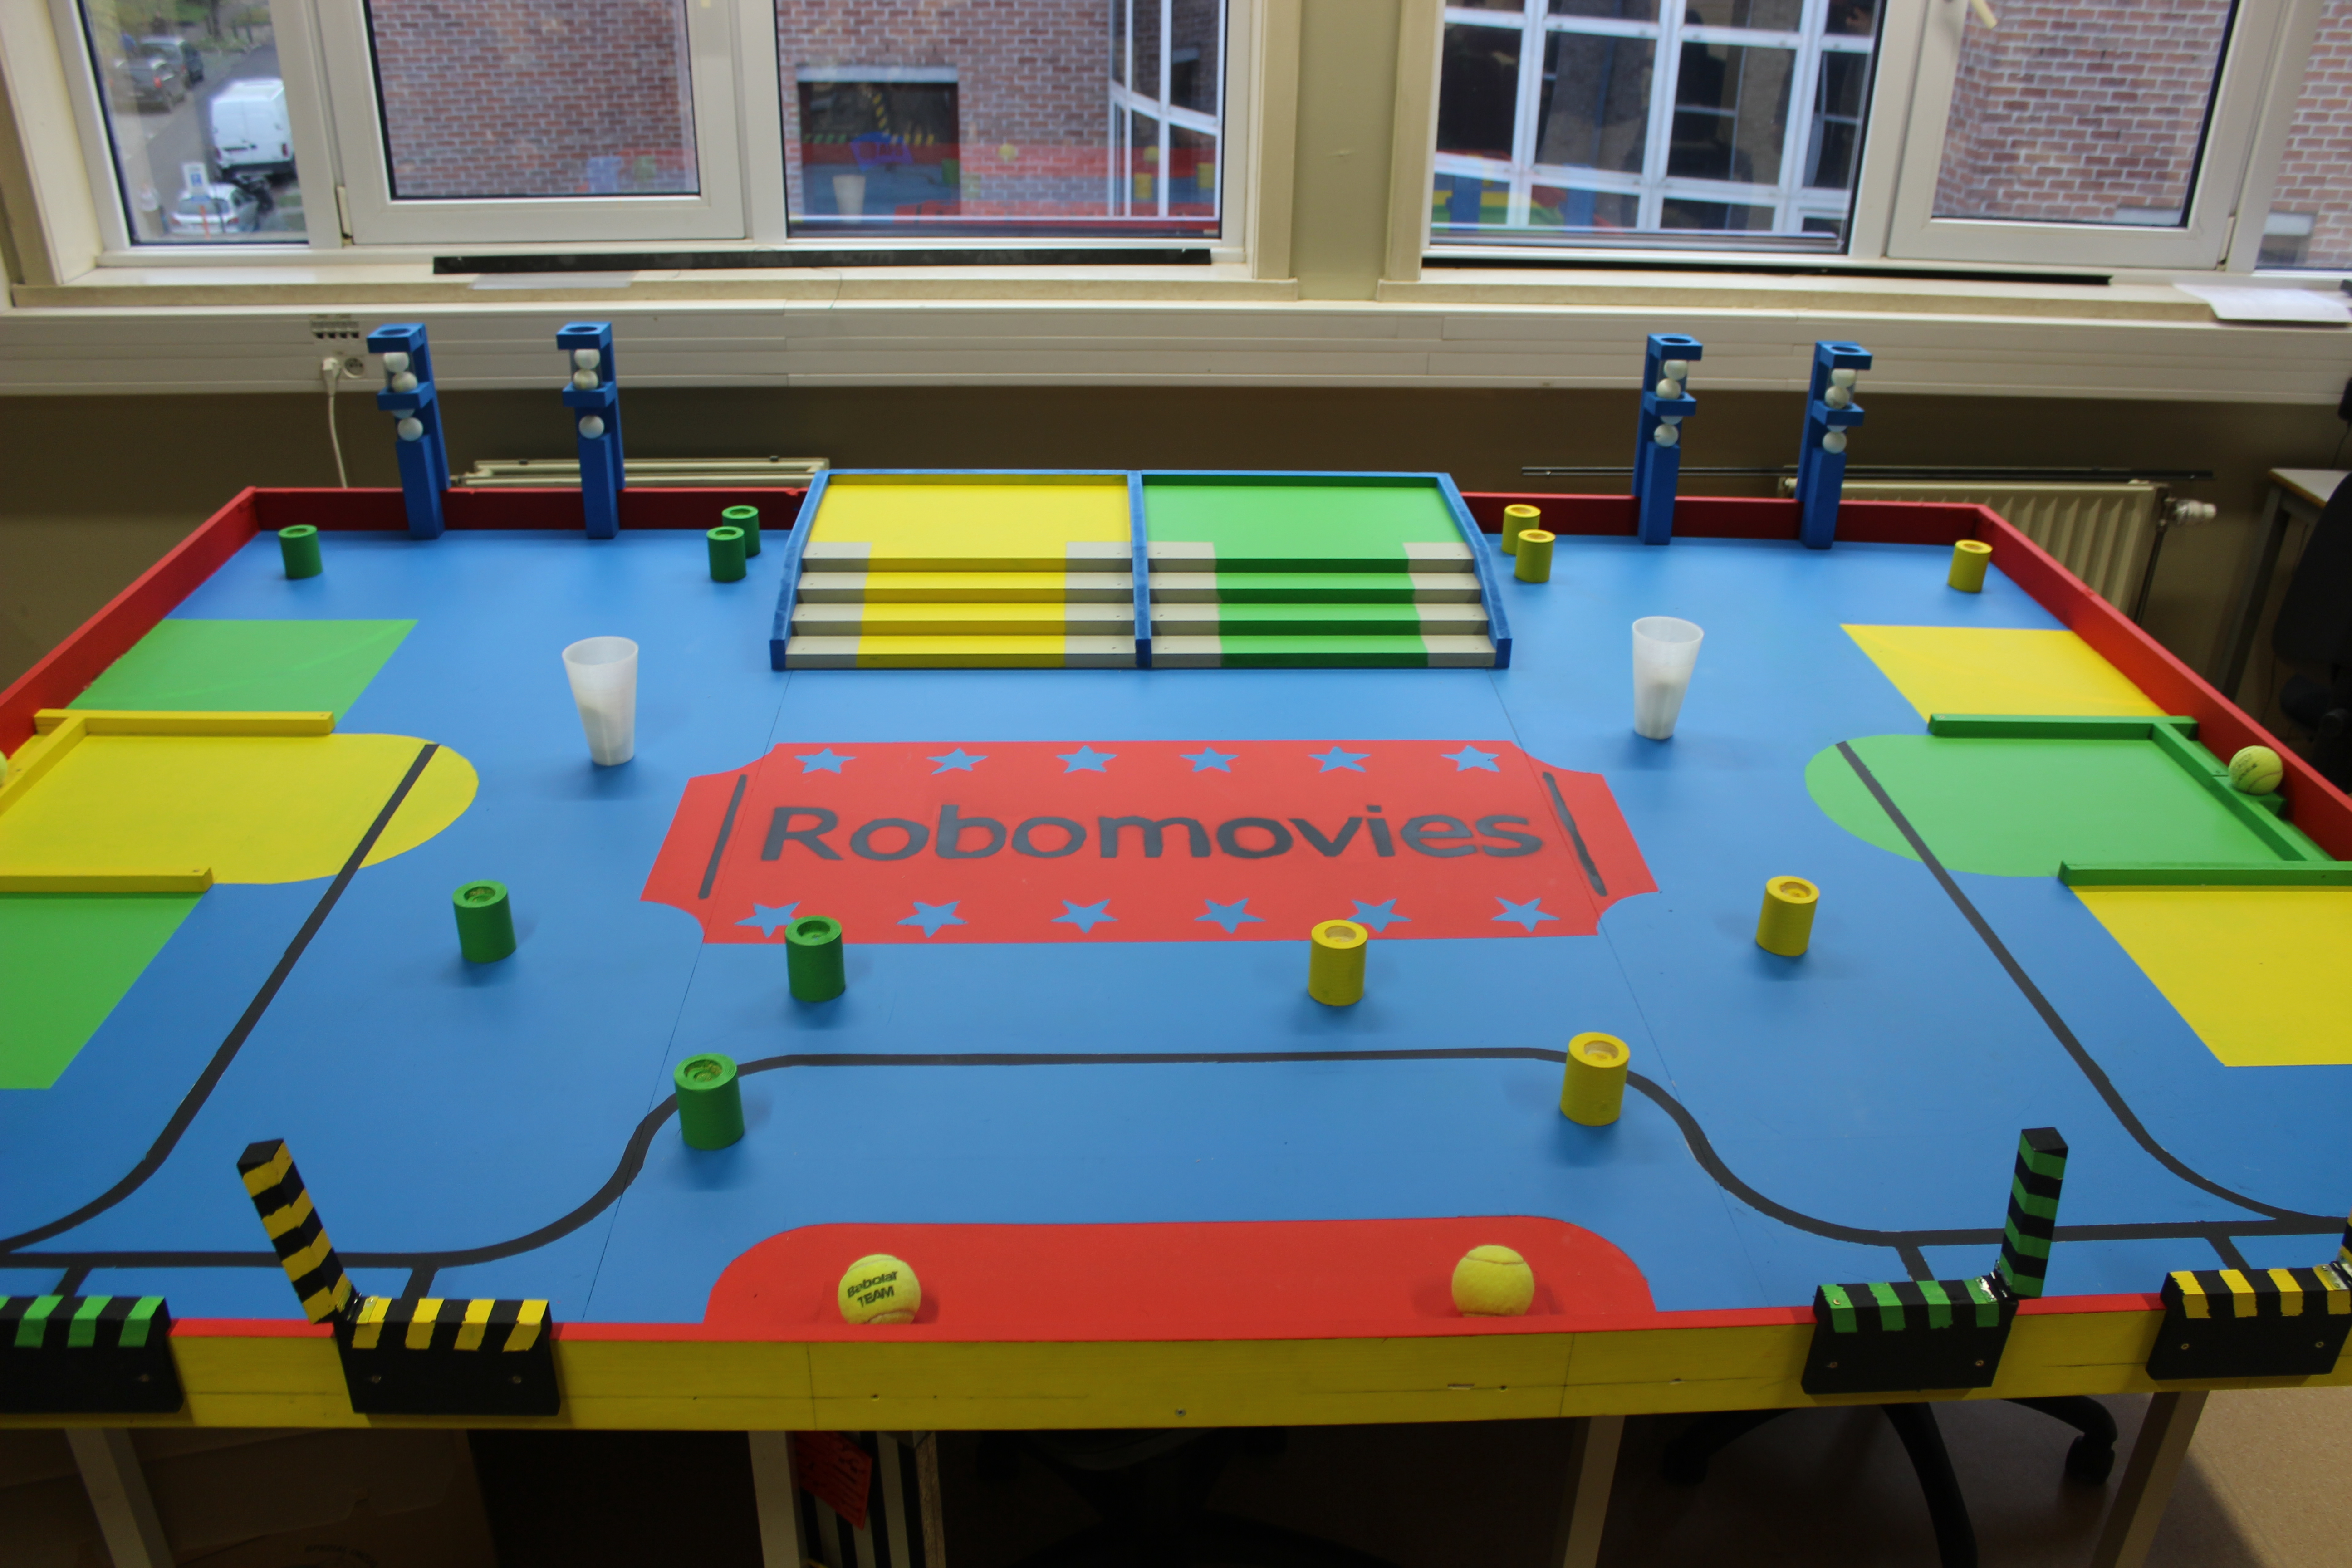
\includegraphics[scale=0.05]{Eurobot_Table_1.JPG}
	\caption{Table}
\end{figure}
\end{frame}

\begin{frame}
\frametitle{Table et actions à réaliser}
\framesubtitle{Action à réaliser}
\begin{itemize}
	\item The spotlight;
	\item The clapperboards;
	\item The popcorn;
	\item Climbing the red carpet steps;
	\item The red carpet.
\end{itemize}
\end{frame}